\documentclass[
	% -- opções da classe memoir --
	12pt,				% tamanho da fonte
	openright,			% capítulos começam em pág ímpar (página vazia se preciso)
% 	twoside,			% para impressão em recto e verso.
    oneside,
	a4paper,			% tamanho do papel. 
	% -- opções da classe abntex2 --
	chapter=TITLE,
 	section=TITLE,
% 	subsection=Title,
% 	subsubsection=Title,
	% -- opções do pacote babel --
	english,			% idioma adicional para hifenização
% 	french,				% idioma adicional para hifenização
% 	spanish,			% idioma adicional para hifenização
	brazil				% o último idioma é o principal do documento
	]{abntex2}

% ---
% Pacotes básicos 
% ---
%\usepackage{lmodern}		% Usa a fonte Latin Modern			
\usepackage{helvet}		% Usa a fonte Arial
\renewcommand{\familydefault}{\sfdefault}

\usepackage[T1]{fontenc}	% Selecao de codigos de fonte.
\usepackage[utf8]{inputenc}	% Codificacao do documento 
\usepackage{indentfirst}	% Indenta o primeiro parágrafo de cada seção.
\usepackage{color}			% Controle das cores
\usepackage{graphicx}		% Inclusão de gráficos
\usepackage{microtype} 		% para melhorias de justificação
\usepackage{setspace}       % para espacamento simples no resumo
\usepackage{pdfpages}
% ---

% ---
% Pacotes adicionais, usados apenas no exemplo
% ---
\usepackage{lipsum} % para geração de dummy text
%\usepackage[utf8]{inputenc}
%\usepackage[T1]{fontenc}
%\usepackage[brazil]{babel} 
% ---

% ---
% Pacotes de citações
% ---
%\usepackage[brazilian,hyperpageref]{backref} % Mostra a página onde cada citação foi feita
%\usepackage[num,abnt-etal-list=0,bibjustif]{abntex2cite} % Citações numéricas (ordem de apresentação)
\usepackage[alf,abnt-etal-list=3,bibjustif,abnt-repeated-author-omit=yes,abnt-repeated-author-omit=yes,abnt-url-package=hyperref,abnt-emphasize=bf]{./abntex2cite} % Citações autor-data (ordem alfabética)

% --- 
% CONFIGURAÇÕES DE PACOTES
% --- 

% % ---
% % Configurações do pacote backref, SE FOR USAR DESCOMENTE TODO ESSE TRECHO
% % Usado sem a opção hyperpageref de backref
% \renewcommand{\backrefpagesname}{Citado na(s) página(s):~}
% % Texto padrão antes do número das páginas
% \renewcommand{\backref}{}
% % Define os textos da citação
% \renewcommand*{\backrefalt}[4]{
% 	\ifcase #1 %
% 		Nenhuma citação no texto.%
% 	\or
% 		Citado na página #2.%
% 	\else
% 		Citado #1 vezes nas páginas #2.%
% 	\fi}%
% % ---


% ---
% Informações de dados para CAPA e FOLHA DE ROSTO
% ---
\usepackage{abntex2esao}
\usepackage[T1]{fontenc}
\usepackage[utf8]{inputenc}
\DeclareUnicodeCharacter{200B}{{\hskip 0pt}}
% ---

%------------
%Outro Idioma
%------------
\usepackage{ifthen}
\RequirePackage{ifthen}
\newif\ifen
\newif\ifpt
\newif\ifes
\newif\iffr
\newif\ifita
\newcommand{\en}[1]{\ifen#1\fi}
\newcommand{\pt}[1]{\ifpt#1\fi}
\newcommand{\es}[1]{\ifes#1\fi}
\newcommand{\fr}[1]{\iffr#1\fi}
\newcommand{\ita}[1]{\ifita#1\fi}
\newcommand{\jan}{%
    \en{January}%
    \pt{Janeiro}%
    \es{Enero}%
    \fr{Janvier}%
    \ita{Gennaio}%
}
\pttrue

%\usepackage{caption}
%\usepackage{subcaption}



% ---
% EXEMPLO PARA CURSO DE POS GRADUAÇÃO
% ---

% \instituicao{Instituto Militar de Engenharia}
% \programapgdepartamento{Engenharia de Transportes}
% \nivelestudo{Pós-Graduação Lato Sensu} % Pós-Graduação Lato Sensu ou Mestrado
% % ---
% \titulo{Modelo Canônico de Trabalho Acadêmico com \abnTeX\space \versaoDocumento}
% \palavraschave{signal,signals company,comunicações nas grandes,apoio de comunicações}
% \keywords{unmanned systems,unmanned vehicles,uav,uas,cooperative tasks,intelligent agents}
% % ---
% \autores{Fulano de}{Silva}% 1+ autores
% % \autor{Fulano de}{Tal} %{nome}{sobrenome}
% \orientadores{Sicrano,Beltrano}{Santos,Oliveira}{Ph.D.,D.Sc.}%{nomes}{sobrenomes}{títulos}
% % ---
% \local{Rio de Janeiro}
% \data{2022}
% \datadefesa{09 de setembro de 2022}
% \bancadeexaminadores{
%     Prof. \textbf{Orientador 1} - D.Sc. da EsAO - Presidente,
%     Prof. \textbf{Orientador 2} - D.Sc. da ECEME,
%     Prof. \textbf{Professor 1} - Oficial QEMA da EsAO,
%     Prof. \textbf{Professor 2} - D.Sc. da EsAO,
% }

% ---



% ---
% EXEMPLO PARA PROJETO DE FIM DE CURSO
% ---

\instituicao{Escola de Aperfeiçoamento de Oficiais}
\programapgdepartamento{Ciências Militares}
\nivelestudo{Pós-Graduação Lato Sensu} % Pós-Graduação Lato Sensu ou Mestrado
% ---
\titulo{O Título do Meu Trabalho}
\palavraschave{comando e controle,apoio a decisão,comunicações}
\keywords{command and control,decision support,signals}
% ---
\autores{Fulano}{de Tal}% {nome}{sobrenome} 1+
\orientadores{Ciclano da Silva}{Souza}{Maj Inf}%{nomes}{sobrenomes}{títulos} 1+
% ---
\local{Rio de Janeiro}
\data{2022}
\datadefesa{9 de setembro de 2022}
\bancadeexaminadores{
     FULANO DA SILVA \textbf{SOUZA} - Maj\\ Escola de Aperfeiçoamento de Oficiais\\ Presidente,
     \textbf{BELTRANO} DA SILVA - Maj\\ Escola de Aperfeiçoamento de Oficiais\\ Membro,
     \textbf{CICLANO} SMITH - Cap\\ Escola de Aperfeiçoamento de Oficiais\\ Membro
}

% ---


% ---
% Configurações de aparência do PDF final

% % alterando o aspecto da cor azul
% \definecolor{blue}{RGB}{41,5,195}

% % informações do PDF
\makeatletter
\hypersetup{
    %pagebackref=true,
    % pdftitle={\@title}, 
    % pdfauthor={\@author},
    % pdfsubject={\imprimirpreambulo},
    % pdfcreator={LaTeX with abnTeX2},
    colorlinks=true, % false: boxed links; true: colored links
    linkcolor=black, % color of internal links
    citecolor=black,	% color of links to bibliography
    filecolor=black, % color of file links
    urlcolor=black,
    bookmarksdepth=4
}
\makeatother
% % --- 
% % --- 



% ---
% Posiciona figuras e tabelas no topo da página quando adicionadas sozinhas
% em um página em branco. Ver https://github.com/abntex/abntex2/issues/170
\makeatletter
\setlength{\@fptop}{5pt} % Set distance from top of page to first float
\makeatother
% ---

% ---
% Possibilita criação de Quadros e Lista de quadros.
% Ver https://github.com/abntex/abntex2/issues/176
%
\newcommand{\quadroname}{Quadro}
\newcommand{\listofquadrosname}{Lista de quadros}

\newfloat[chapter]{quadro}{loq}{\quadroname}
\newlistof{listofquadros}{loq}{\listofquadrosname}
\newlistentry{quadro}{loq}{0}

% configurações para atender às regras da ABNT
\setfloatadjustment{quadro}{\centering}
\counterwithout{quadro}{chapter}
\renewcommand{\cftquadroname}{\quadroname\space} 
\renewcommand*{\cftquadroaftersnum}{\hfill--\hfill}

\setfloatlocations{quadro}{hbtp} % Ver https://github.com/abntex/abntex2/issues/176
% ---

% --- 
% Espaçamentos entre linhas e parágrafos 
% --- 

% O tamanho do parágrafo é dado por:
\setlength{\parindent}{1.3cm}

% Controle do espaçamento entre um parágrafo e outro:
\setlength{\parskip}{0.2cm}  % tente também \onelineskip

% ---
% compila o indice
% ---
\makeindex
% ---
%
%    \usepackage{fancyhdr}
%    \pagestyle{fancy}
%    \renewcommand{\headrulewidth}{0pt}
%    \fancyhf{}
%    \cfoot{\noindent\fcolorbox{red}{white}{\parbox{\dimexpr \linewidth-2\fboxsep-2\fboxrule}{%
%                \centering{\color{red}{\textbf{INFORMAÇÃO DE P\&D - ACESSO RESTRITO}\\
%                        §1º do Art. 7º da Lei nº 12.527, de 18 de novembro de 2011\\
%                        Inciso II do Art. 6º do Decreto nº 7.724, de 16 de maio de 2012}}}}}
%

% Marca dagua com o reservado
%\usepackage{draftwatermark} 
%\SetWatermarkColor[rgb]{1,0,0}
%\SetWatermarkAngle{0}
%\SetWatermarkText{\textsc{RESERVADO}}
%\SetWatermarkScale{0.12}
%\SetWatermarkVerCenter{10mm}
%\SetWatermarkHorCenter{150mm}

% acronyms
\usepackage{acro} 
%\acsetup{
%    list/display=used ,
%    list/heading=none
%}
%\DeclareAcronym{xxxxx}{short={xxxxxxxxx},long={xxxxxxxxxxxxx}}
\DeclareAcronym{C²}{short={C²},long={Comando e Controle}}
\DeclareAcronym{END}{short={END},long={Estratégia Nacional de Defesa}}
\DeclareAcronym{EMCFA}{short={EMCFA},long={Estado-Maior Conjunto das Forças Armadas}}
\DeclareAcronym{GU}{short={GU},long={Grande Unidade}}
\DeclareAcronym{SAD}{short={SAD},long={Sistemas de Apoio à Decisão}}
\DeclareAcronym{SI}{short={SI},long={Sistemas de Informação}}
\DeclareAcronym{SISBIN}{short={SISBIN},long={Sistema Brasileiro de Inteligência}}
\DeclareAcronym{SISNACC}{short={SISNACC},long={Sistema Nacional de Comunicações Críticas}}
\DeclareAcronym{TIC}{short={TIC},long={Tecnologia da Informações e Comunicações}}
\DeclareAcronym{SisMC²}{short={SisMC²},long={Sistema Militar de Comando e Controle}}
\DeclareAcronym{CONOPS}{short={CONOPS},long={Conceito Operacional}}
\DeclareAcronym{TI}{short={TI},long={Tecnologia da Informação}}
\DeclareAcronym{MD}{short={MD},long={Ministério da Defesa}}
\DeclareAcronym{OMs}{short={OMs},long={Organizações Militares}}

% ----
% Início do documento
% ----
\begin{document}
    
% Seleciona o idioma do documento (conforme pacotes do babel)
%\selectlanguage{english}
\selectlanguage{brazil}

% Retira espaço extra obsoleto entre as frases.
\frenchspacing 

% ----------------------------------------------------------
% ELEMENTOS PRÉ-TEXTUAIS
% ----------------------------------------------------------
% \pretextual

% ---
% Capa
% ---
\imprimircapa
% ---

% ---
% Folha de rosto
% (o * indica que haverá a ficha bibliográfica)
% ---
\imprimirfolhaderosto*
% ---

% ---
% Inserir a ficha bibliografica
% ---

% \begin{fichacatalografica}
%     \includepdf{fig_ficha_catalografica.pdf}
% \end{fichacatalografica}

\imprimirfichacatalografica
% ---

% ---
% Inserir folha de aprovação
% ---

% \begin{folhadeaprovacao}
% \includepdf{folhadeaprovacao_final.pdf}
% \end{folhadeaprovacao}
%
\imprimirfolhadeaprovacao
% ---

% ---
% Dedicatória
% ---
\begin{dedicatoria}
   \vspace*{\fill}
   \centering
   \noindent
   \textit{ Este trabalho é dedicado aos xxxxxxxxxxxx, que assim como eu encerram uma difícil etapa da vida acadêmica. Dedico este trabalho a todo xxxxxxxxxxxxx, corpo docente e discente, a quem fico lisonjeado por dele ter feito parte.} \vspace*{\fill}
\end{dedicatoria}
% ---

% ---
% Agradecimentos
% ---
\begin{agradecimentos}
\lipsum[2]



\end{agradecimentos}
% ---

% ---
% Epígrafe
% ---
\begin{epigrafe}
    \vspace*{\fill}
	\begin{flushright}
		\textit{``Não vos amoldeis às estruturas deste mundo, \\
		mas transformai-vos pela renovação da mente, \\
		a fim de distinguir qual é a vontade de Deus: \\
		o que é bom, o que Lhe é agradável, o que é perfeito.\\
		(Bíblia Sagrada, Romanos 12, 2)}
	\end{flushright}
\end{epigrafe}
% ---

% ---
% RESUMOS
% ---

% resumo em português
\setlength{\absparsep}{18pt} % ajusta o espaçamento dos parágrafos do resumo
\begin{resumo}
\SingleSpacing
%destacar o assunto do trabalho, o objetivo, o método e os resultados esperados. Deve apresentam de 150 a 200 palavras, escritas em formato de bloco,espaço simples e fonte menor (um  ponto) que a do texto do projeto
 \lipsum[1]

 Palavras-chave: \imprimirpalavraschave
\end{resumo}

% resumo em inglês
\begin{resumo}[Abstract]
 \begin{otherlanguage*}{english}
%  \linespread{1.3}
\SingleSpacing
 \lipsum[3]
   \vspace{\onelineskip}
 
   \noindent 
   Keywords: \imprimirkeywords
 \end{otherlanguage*}
\end{resumo}

% ---
% inserir lista de ilustrações
% ---
\pdfbookmark[0]{\listfigurename}{lof}
\listoffigures*
\cleardoublepage
% ---

% ---
% inserir lista de quadros
% ---
%\pdfbookmark[0]{\listofquadrosname}{loq}
%\listofquadros*
%\cleardoublepage
% ---

% ---
% inserir lista de tabelas
% ---
%\pdfbookmark[0]{\listtablename}{lot}
%\listoftables*
%\cleardoublepage
% ---

% ---
% inserir lista de abreviaturas e siglas
% ---
\begin{siglas}
    \item
    \printacronyms[heading=none]
%    \printacronyms[display=used,heading=none]
\end{siglas}
% ---

% ---
% inserir lista de símbolos
% ---
%\begin{simbolos}
%  \item[$ \Gamma $] Letra grega Gama
%  \item[$ \Lambda $] Lambda
%\end{simbolos}
% ---

% ---
% inserir o sumario
% ---

\makeatletter
\let\oldcontentsline\contentsline
\def\contentsline#1#2{%
    \oldcontentsline{#1}{\MakeTextUppercase{#2}}%
}
\makeatother

\pdfbookmark[0]{\contentsname}{toc}
\tableofcontents*
\cleardoublepage
% ---

% ----------------------------------------------------------
% ELEMENTOS TEXTUAIS
% ----------------------------------------------------------
\textual

% ----------------------------------------------------------
% Introdução (exemplo de capítulo sem numeração, mas presente no Sumário)
% ----------------------------------------------------------
\chapter{Introdução}
% ----------------------------------------------------------

\lipsum[3] \cite{LivroBrancodeDefesaNacional455}.

\lipsum[4] \cite{PoliticaNacionaldeDefesaeEstrategiaNacionaldeDefesa457,LivroBrancodeDefesaNacional455}.

\lipsum[5] \cite{LivroBrancodeDefesaNacional455}.

\lipsum[6] \cite{PoliticaNacionaldeDefesaeEstrategiaNacionaldeDefesa457}.

\lipsum[7] \cite{PoliticaNacionaldeDefesaeEstrategiaNacionaldeDefesa457}.

\lipsum[8-10]

\section{Problema}

\lipsum[11-13] \cite{ConceitoOperacionaldoSistemadeInformacaoedeApoioaDecisaoparaComandoeControle492}.


\section{Objetivos}
\lipsum[14]

\subsection{Objetivo Geral}
\lipsum[15]

\subsection{Objetivos Específicos}
\begin{itemize}
    \item xxxxxxxxxxxxxxxxxx
    \item xxxxxxxxxxxxxxxx \ac{SAD} xxxxxxxxxxxxxxx \ac{SisMC²}; e
    \item xxxxxxxxxxxx \ac{SAD} xxxxxxxxxxxxxxxxxxxxxxx.
\end{itemize}


\chapter{Referencial Teórico}
\noindent
\lipsum[15]

\section{Generalidades}

\lipsum[16]

\subsection{Conceitos da xxxxxxxxxxxxxx}

\begin{citacao}
    \lipsum[17] \cite{DoutrinaMilitarTerrestre54}.
\end{citacao}

Segundo \citeonline{DoutrinaMilitarTerrestre54} xxxxxxxxxxxxxxxxxxxxxxxxx xxxxxxxxxx xxxxxxxxx.

\begin{citacao}
    \lipsum[18] \cite{DoutrinaMilitarTerrestre54}.
\end{citacao}

\lipsum[19]



\section{Principais xxxxxxxxxx em uso na FTer}
\lipsum[20-23] \cite{LivroBrancodeDefesaNacional455,EstruturaMilitardeDefesa454}.


\section{Sistema xxxxxxxx xxxxxxxx}

\lipsum[7]


\section{Aplicações xxxxxxxxxxxxxxxx}

\lipsum[24]

\begin{figure}[!h]
    \centering
    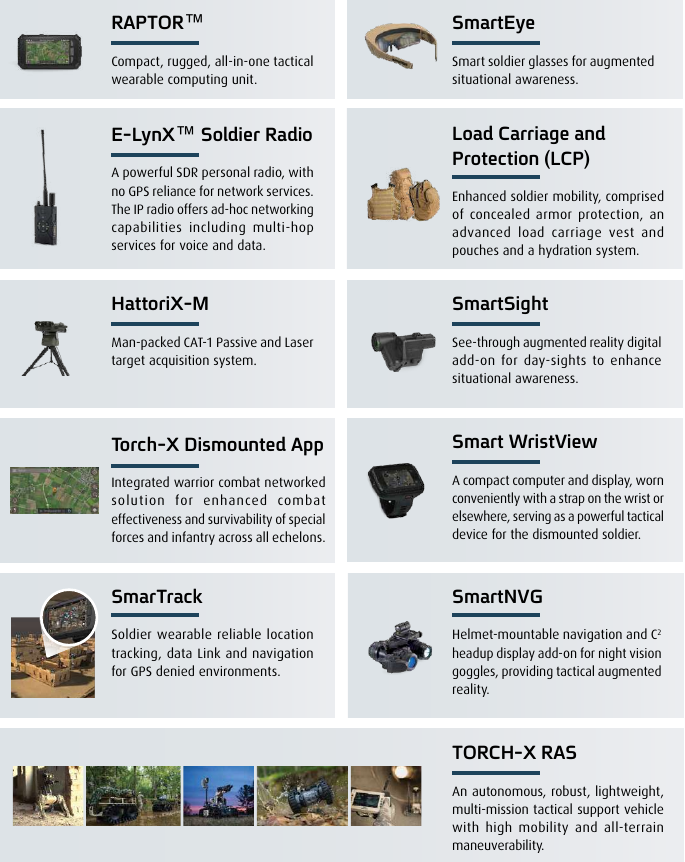
\includegraphics[width=1\linewidth]{img/torchx_dismounted}
    \caption{Datasheet do Torch X dismounted com os principais elementos integradores do sistema.}
    \legend{Fonte: \cite{TorchXDs}}
    \label{fig:torchxdismounted}
\end{figure}

\lipsum[25]

\begin{figure}[!h]
    \centering
    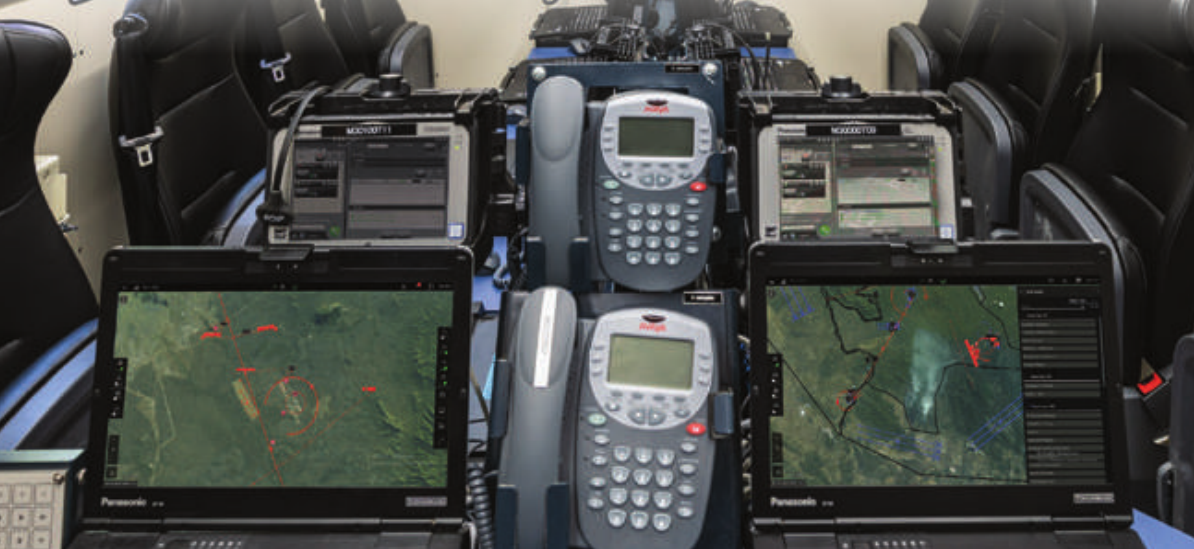
\includegraphics[width=1\linewidth]{img/torchx}
    \caption{Torch X HQ em operação}
    \legend{Fonte: \cite{TorchXHQ}}
    \label{fig:torchxhd}
\end{figure}

\lipsum[26]

\begin{figure}[!h]
    \centering
    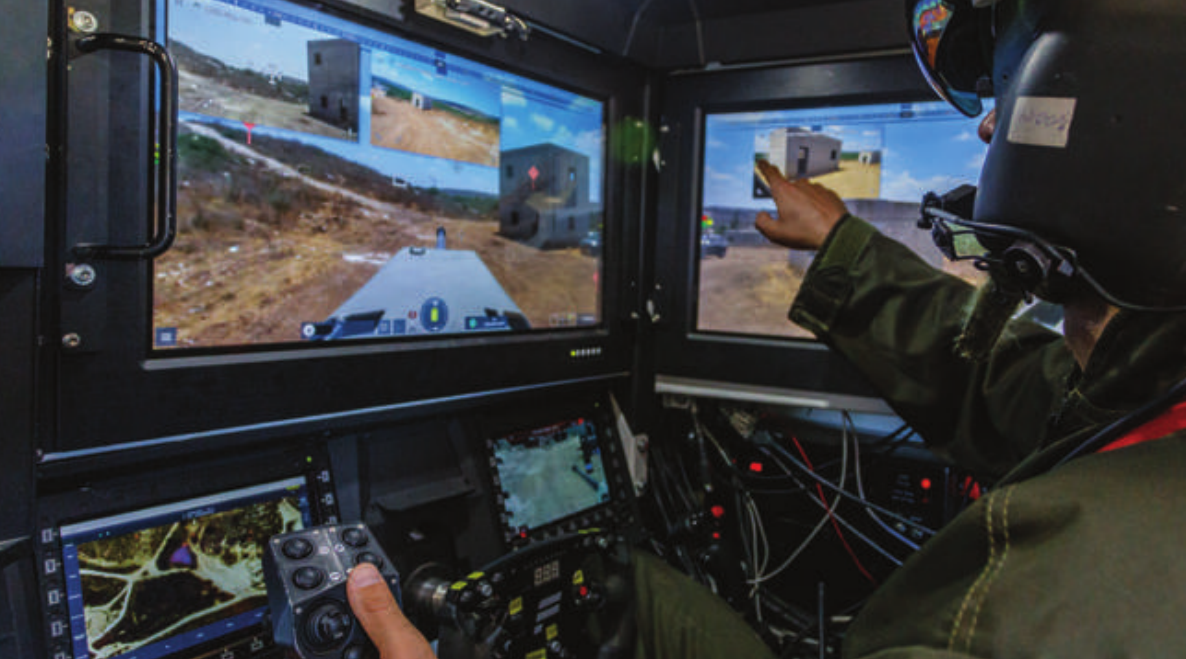
\includegraphics[width=1\linewidth]{img/torchx_mounted}
    \caption{Torch X Mounted}
    \legend{Fonte: \cite{TorchX}}
    \label{fig:torchxmounted}
\end{figure}

\lipsum[27]

\section{xxxxxxxx xxxxxxxxxxxxx}

\subsection{Conceitos de xxxxxxxx}

\lipsum[25-30]

\begin{equation}
    \label{math:acuracia}
    AccC_1 = \frac{VP + VN}{n}
\end{equation}


\begin{equation}
    \label{math:abrangencia}
    RevC_1 = \frac{VP}{VP+FN}
\end{equation}



\begin{equation}
    \label{math:precisao}
    PrecC_1 = \frac{VP}{VP+FP}
\end{equation}


\begin{equation}
    \label{math:f1}
    F_1 = \frac{2*Prec*Rev}{Prec + Rev}
\end{equation}

\lipsum[31]

\begin{table}[!ht]
    \centering
    \caption{Matriz de xxxxxxxxx}
    \label{tab:matriz_de_xxxxxx}
    \vspace{0.5cm}
    \begin{tabular}{r|cccc||c}
        & P ($ C_1 $)   & P ($ C_2 $)   & Total Real \\
        \hline
        \hline
        R ($ C_1 $)             & (VP) 120 & (FN) 40  & 160      \\
        R ($ C_2 $)             & (FP) 33  & (VN) 127 & 160      \\
        \hline
        \hline
        Total xxxxxx & 153 & 167 & 320      \\
        \hline
    \end{tabular}
\end{table}

\chapter{Metodologia}

\section{Objeto Formal de Estudo}
\lipsum[32]

\section{Delineamento da Pesquisa}
\lipsum[33]

\subsection{Procedimentos para revisão da literatura}
\label{procedimentosMetd}
\lipsum[34]

\subsection{Procedimentos Metodológicos}
\lipsum[35]

\subsection{Instrumentos}
\lipsum[36]

\subsection{Análise de Dados}
\lipsum[37]

\section{Justificativa}
\lipsum[38-42]
\chapter{Resultados}\label{cap_trabalho_academico}

\lipsum[43-49]
\chapter{Discussao dos Resultados}\label{cap_trabalho_academico}

\lipsum[56-60]
% ---
% Conclusão
% ---
\chapter{Conclusão}
% ---

\lipsum[50-55] 


% ----------------------------------------------------------
% ELEMENTOS PÓS-TEXTUAIS
% ----------------------------------------------------------
\postextual
% ----------------------------------------------------------

% ----------------------------------------------------------
% Referências bibliográficas
% ----------------------------------------------------------
\bibliography{refs.bib}

% ----------------------------------------------------------
% Apêndices
% ----------------------------------------------------------
%\begin{apendicesenv}
%    \partapendices
%    \chapter{Apêndice Exemplo}

Curabitur tortor. Pellentesque nibh. Aenean quam. In scelerisque sem at dolor. Maecenas mattis. Sed convallis tristique sem. Proin ut ligula vel nunc egestas porttitor. Morbi lectus risus, iaculis vel, suscipit quis, luctus non, massa. Fusce ac turpis quis ligula lacinia aliquet. Mauris ipsum. Nulla metus metus, ullamcorper vel, tincidunt sed, euismod in, nibh. Quisque volutpat condimentum velit.

Class aptent taciti sociosqu ad litora torquent per conubia nostra, per inceptos himenaeos. Nam nec ante. Sed lacinia, urna non tincidunt mattis, tortor neque adipiscing diam, a cursus ipsum ante quis turpis. Nulla facilisi. Ut fringilla. Suspendisse potenti. Nunc feugiat mi a tellus consequat imperdiet. Vestibulum sapien. Proin quam. Etiam ultrices. Suspendisse in justo eu magna luctus suscipit. Sed lectus. Integer euismod lacus luctus magna.

Lorem ipsum dolor sit amet, consectetur adipiscing elit. Integer nec odio. Praesent libero. Sed cursus ante dapibus diam. Sed nisi. Nulla quis sem at nibh elementum imperdiet. Duis sagittis ipsum. Praesent mauris. Fusce nec tellus sed augue semper porta. Mauris massa. Vestibulum lacinia arcu eget nulla. Class aptent taciti sociosqu ad litora torquent per conubia nostra, per inceptos himenaeos. Curabitur sodales ligula in libero. Sed dignissim lacinia nunc.

\chapter{Apêndice Exemplo 02}

Curabitur tortor. Pellentesque nibh. Aenean quam. In scelerisque sem at dolor. Maecenas mattis. Sed convallis tristique sem. Proin ut ligula vel nunc egestas porttitor. Morbi lectus risus, iaculis vel, suscipit quis, luctus non, massa. Fusce ac turpis quis ligula lacinia aliquet. Mauris ipsum. Nulla metus metus, ullamcorper vel, tincidunt sed, euismod in, nibh. Quisque volutpat condimentum velit.

Class aptent taciti sociosqu ad litora torquent per conubia nostra, per inceptos himenaeos. Nam nec ante. Sed lacinia, urna non tincidunt mattis, tortor neque adipiscing diam, a cursus ipsum ante quis turpis. Nulla facilisi. Ut fringilla. Suspendisse potenti. Nunc feugiat mi a tellus consequat imperdiet. Vestibulum sapien. Proin quam. Etiam ultrices. Suspendisse in justo eu magna luctus suscipit. Sed lectus. Integer euismod lacus luctus magna.

Lorem ipsum dolor sit amet, consectetur adipiscing elit. Integer nec odio. Praesent libero. Sed cursus ante dapibus diam. Sed nisi. Nulla quis sem at nibh elementum imperdiet. Duis sagittis ipsum. Praesent mauris. Fusce nec tellus sed augue semper porta. Mauris massa. Vestibulum lacinia arcu eget nulla. Class aptent taciti sociosqu ad litora torquent per conubia nostra, per inceptos himenaeos. Curabitur sodales ligula in libero. Sed dignissim lacinia nunc.


\chapter{Quisque libero justo}

\lipsum[50]


\chapter{Nullam elementum urna vel imperdiet sodales elit ipsum pharetra ligula ac pretium ante justo a nulla curabitur tristique arcu eu metus}

\lipsum[54-56]
%\end{apendicesenv}
% ---

% ----------------------------------------------------------
% Anexos
% ----------------------------------------------------------
%\begin{anexosenv}
%    \partanexos
%    \chapter{Anexo Exemplo}

\lipsum[3-9]

\chapter{Anexo Exemplo 02}

\lipsum[1-4]


\chapter{Morbi ultrices rutrum lorem.}

\lipsum[29-30]


\chapter{Cras non urna sed feugiat cum sociis natoque penatibus et magnis dis parturient montes nascetur ridiculus mus}

\lipsum[31-32]

\chapter{Fusce facilisis lacinia dui}

\lipsum[32-36]
%\end{anexosenv}

%---------------------------------------------------------------------
% INDICE REMISSIVO
%---------------------------------------------------------------------
\phantompart
\printindex
%---------------------------------------------------------------------

\end{document}
